\documentclass[twocolumn,secnumarabic,amssymb,nobibnotes,aps,prl,superscriptaddress,10pt]{revtex4-2}

\usepackage{graphicx}
\usepackage{amsmath,amssymb,bm}
\usepackage{booktabs}
\usepackage{xcolor}
\usepackage[colorlinks=true,linkcolor=blue!70!black,citecolor=blue!70!black,urlcolor=blue!70!black]{hyperref}

% Nature-style figure labels
\renewcommand{\figurename}{\textbf{Fig.}}
\renewcommand{\thefigure}{\textbf{\arabic{figure}}}

% editorial check marks: where the draft differs from the repository notes (see report/README.md, Appendix)
\newcommand{\note}[1]{{\color{red}\small[#1]}}

\begin{document}

\title{Non-stoichiometric superionic ice and deep hydrogen sequestration in ice giants}

\author{Victor Naden Robinson}
\affiliation{School of Chemistry, University of Nottingham, University Park, Nottingham NG7 2RD, UK}

\date{\today}

\begin{abstract}
\noindent\textbf{Water is the primary constituent of the deep mantles of Uranus, Neptune and volatile-rich sub-Neptune exoplanets, where megabar pressures ($100\text{--}600\text{ GPa}$) and temperatures of $3,000\text{--}7,000\text{ K}$ stabilize superionic ice---a state of matter in which oxygen ions form a rigid crystalline lattice while protons diffuse like a liquid. Planetary interior models universally assume that this crystalline superionic mantle is strictly stoichiometric ($\text{H}_2\text{O}$) and chemically isolated from the overlying hydrogen--helium envelope below the melting curve. Here we show, using machine-learning-accelerated thermodynamic integration and ghost-proton insertion anchored to first-principles density functional theory, that face-centred cubic (fcc) superionic ice spontaneously dissolves substantial excess hydrogen to form a non-stoichiometric solid solution, $\text{H}_{2+x}\text{O}$, with equilibrium concentrations of $x \approx 0.03\text{--}0.10$ near the melting line. Whereas proton incorporation is enthalpically repulsive at low temperatures, the indistinguishability of inserted and host protons within the mobile superionic sublattice eliminates the logarithmic configurational chemical potential singularity, enabling high-temperature entropic stabilization of interstitial hydrogen. This non-stoichiometry depresses the superionic melting curve, broadens the solid--liquid transition into a compositional mushy zone, and establishes the solid mantle as a massive deep reservoir of planetary hydrogen. As an ice giant cools over gigayears, secular decreases in hydrogen solubility drive upward exsolution of buoyant hydrogen, providing a unified compositional mechanism to stratify heat flow in Uranus and power multipolar planetary dynamos.}
\end{abstract}

\maketitle

\section*{Introduction}

The internal structures, thermal evolution and magnetic field generation of the solar system's ice giants---Uranus and Neptune---as well as the abundant population of sub-Neptune exoplanets, are governed by the high-pressure phase behaviour of water and its mixtures with light volatiles\cite{Guillot2005,Helled2020}. In standard three-layer planetary models, an outer molecular hydrogen--helium ($\text{H}_2\text{--He}$) atmosphere overlies a deep mantle dominated by ``ices'' ($\text{H}_2\text{O}$, $\text{NH}_3$ and $\text{CH}_4$) spanning pressures from $20\text{ GPa}$ to $600\text{ GPa}$ and temperatures from $2,000\text{ K}$ to $7,000\text{ K}$. Shock-compression experiments\cite{Millot2018,Millot2019}, static diamond-anvil cell X-ray diffraction\cite{Prakapenka2021} and first-principles molecular dynamics simulations\cite{Cavazzoni1999,Wilson2013,Cheng2021} have established that across much of this mantle regime, water exists as superionic ice (specifically the body-centred cubic, bcc, and face-centred cubic, fcc, Ice XVIII phases), wherein oxygen ions occupy crystallographic lattice sites while protons hop rapidly through interstitial channels.

Above the superionic melting curve, fluid $\text{H}_2\text{O}$ and fluid $\text{H}_2$ become completely miscible at megabar pressures\cite{Soubiran2015}. Below the melting curve, however, phase-diagram and planetary-interior models have universally treated crystalline superionic ice as a strictly line-compound stoichiometric phase ($\text{H}_2\text{O}$). Under this assumption, freezing of the superionic mantle completely expels molecular hydrogen into the overlying fluid envelope. Yet this strict stoichiometric boundary leaves fundamental planetary observations unresolved: most notably, the striking luminosity dichotomy between Uranus (which radiates virtually no excess internal heat) and Neptune (which radiates more than twice the solar energy it absorbs)\cite{Pearl1991,Nettelmann2013}, as well as the requirement for a thin, convecting, electrically conducting shell above a stably stratified interior to generate their non-dipolar, multipolar magnetic fields\cite{Stanley2004}.

Testing whether crystalline superionic ice can deviate from $\text{H}_2\text{O}$ stoichiometry to form a hydrogen-enriched solid solution ($\text{H}_{2+x}\text{O}$) has remained computationally intractable for direct \textit{ab initio} molecular dynamics (AIMD). Resolving dilute equilibrium defect concentrations ($x = 0.01\text{--}0.10$) requires free-energy precision better than $10\text{ meV/atom}$ across large supercells and nanosecond cumulative trajectories. Moreover, standard harmonic-reference (Frenkel--Ladd) thermodynamic integration (TDI) struggles to capture the communal entropy of diffusing off-stoichiometric species, while direct ghost-particle insertion suffers from severe repulsive core-overlap singularities as the coupling parameter $\lambda \to 0$.

Here we overcome these barriers by combining a fine-tuned Graph Atomic Cluster Expansion (GRACE) machine-learning interatomic potential\cite{Bochkarev2024} with two independent free-energy pathways: (1) polynomial-stretched ghost-proton insertion into superionic fcc $\text{H}_2\text{O}$ hosts ($n = 1, 2, 4$ excess protons) extrapolated to infinite dilution, and (2) direct two-stage Frenkel--Ladd and liquid $\lambda$-switching TDI across stoichiometric and off-stoichiometric $\text{H}_{2+x}\text{O}$ compositions ($0 \le x \le 1$) from $300\text{ GPa}$ to $500\text{ GPa}$ and $3,000\text{ K}$ to $9,000\text{ K}$.

\begin{figure*}[t!]
    \centering
    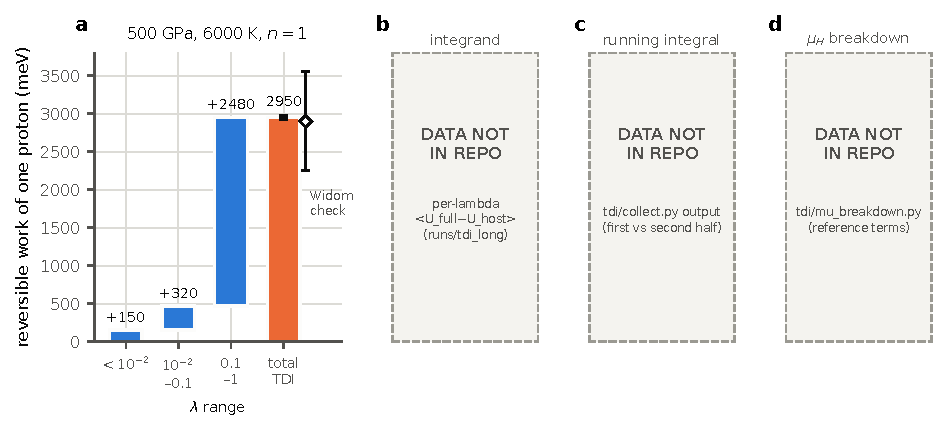
\includegraphics[width=0.95\textwidth]{figures/fig1_insertion.pdf}
    \caption{\textbf{Thermodynamics of ghost-proton insertion in fcc superionic ice.} \textbf{a}, Reversible work of switching on one ghost proton ($n=1$) at $500\text{ GPa}$ and $6,000\text{ K}$, split by coupling range (blue; cumulative bars, $+150$, $+320$ and $+2,480\text{ meV}$ for $\lambda<10^{-2}$, $10^{-2}\text{--}0.1$ and $0.1\text{--}1$) and the total TDI value of $2.95\pm0.02\text{ eV}$ (orange). The diamond is an independent Widom test-particle estimate on the host frames ($2.90\text{ eV}$; block range $2.4\text{--}3.7\text{ eV}$, not converged). \textbf{b--d}, Ensemble-averaged integrand in $\lambda$ and in the stretched coordinate $x_\lambda=\lambda^{1/p}$, running TDI integral, and the complete free-energy decomposition of $\mu_{\text{H}}-G_{\text{H}}^{\text{pure}}$ (repulsive work, thermal de Broglie reference $3k_{\text{B}}T\ln\Lambda$, placement term, pure-H reference): \emph{panels pending, per-$\lambda$ run data are not in the repository}. Values in \textbf{a} are transcribed from the repository notes.}
    \label{fig:insertion}
\end{figure*}

\section*{Thermodynamics of Proton Insertion}

To achieve first-principles accuracy across the entire $\text{H}_2\text{O}\text{--H}$ binary system, we fine-tuned multi-element GRACE models (\texttt{ft\_m2}) against Kohn--Sham DFT calculations spanning compositions from pure $\text{H}_2\text{O}$ through $\text{H}_{2.125}\text{O}$, $\text{H}_{2.25}\text{O}$, $\text{H}_{2.5}\text{O}$, $\text{H}_3\text{O}$, $\text{H}_5\text{O}$, $\text{H}_7\text{O}$ and pure $\text{H}$ across $T = 2,000\text{--}13,000\text{ K}$ and $P = 300\text{--}1,200\text{ GPa}$ (Extended Data Fig.~1). Whereas zero-shot foundation potentials exhibit severe composition-dependent pressure biases exceeding $50\text{ GPa}$, the fine-tuned potential achieves a pressure root-mean-square error (RMSE) of $1.65\text{ GPa}$ and an energy RMSE of $19.6\text{ meV/atom}$ ($0.056\,k_{\text{B}}T$) across the entire validation manifold.\note{check: repo records ft\_m2 validation as energy MAE 18.4 meV/atom, force MAE 511 meV/\AA, stress MAE 2.05 GPa (App.~A2)} Benchmark TDI calculations of the fcc--bcc free-energy difference ($G_{\text{fcc}} - G_{\text{bcc}}$) for pure $\text{H}_2\text{O}$ at $3,000\text{ K}$ and $5,000\text{ K}$ reproduce previous PBE-corrected MLP and direct DFT-TI benchmarks\cite{Wilson2013,Cheng2021} within statistical uncertainty across $100\text{--}500\text{ GPa}$ (Extended Data Fig.~2).

In a conventional crystalline solid, introducing an interstitial defect at dilute concentration $x = n / N_{\text{O}}$ carries a canonical configurational entropy penalty that diverges logarithmically as $\mu_{\text{defect}} \propto k_{\text{B}}T \ln x$. In superionic ice, however, the $N_{\text{H}} = 2N_{\text{O}}$ host protons already form a delocalized, permutationally indistinguishable liquid-like sublattice diffusing through the rigid oxygen framework of volume $V$. When $n$ additional identical protons are inserted into this superionic host, the ideal canonical configurational partition function ratio is governed by

\begin{align}
\Delta F_{\mathrm{id}}(n) &= -k_{\mathrm{B}}T\,\ln\left[\frac{V^{n}}{\Lambda^{3n}}\,\frac{N_{\mathrm{H}}!}{(N_{\mathrm{H}}+n)!}\right]\nonumber\\
&\approx n\,k_{\mathrm{B}}T\left[3\ln\Lambda-\ln\left(\frac{V}{2N_{\mathrm{O}}+n}\right)\right]
\label{eq:placement}
\end{align}

where $\Lambda = h / \sqrt{2\pi m_{\text{H}} k_{\text{B}} T}$ is the thermal de Broglie wavelength. Crucially, because the denominator inside the logarithm is the total mobile proton density $(2N_{\text{O}} + n)/V$ rather than $n/V$, the chemical potential of an inserted proton approaches a finite intercept as $x \to 0$, with a linear ideal mixing slope of $\Delta \mu_{\text{id}}(x) \approx k_{\text{B}}T x / 2$ (or $k_{\text{B}}T x / 4$ for the cumulative per-proton average).

\begin{figure*}[t!]
    \centering
    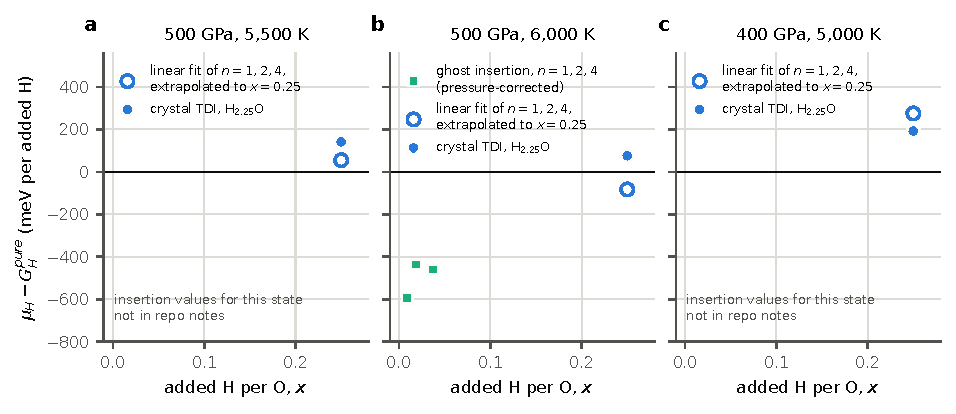
\includegraphics[width=0.95\textwidth]{figures/fig2_solubility.pdf}
    \caption{\textbf{Chemical potential of excess hydrogen across composition.} Excess hydrogen chemical potential $\mu_{\text{H}}-G_{\text{H}}^{\text{pure}}$ per added H versus added H per oxygen ($x$) for three of the state points studied. Green squares: fixed-volume ghost-proton insertion at $n=1,2,4$ ($x=n/108$), pressure-corrected to the target pressure (values read from the repository notes, approximate). Filled blue circles: direct Frenkel--Ladd crystal TDI of $\text{H}_{2.25}\text{O}$ ($x=0.25$). Open blue circles: the repository's linear fit of the $n=1,2,4$ points extrapolated to $x=0.25$. Insertion values for $500\text{ GPa}$/$5,500\text{ K}$ and $400\text{ GPa}$/$5,000\text{ K}$ and the $300\text{--}400\text{ GPa}$, $7,000\text{ K}$ panels of the planned figure are not in the repository. No error bars are shown because the notes quote none for these values.}
    \label{fig:solubility}
\end{figure*}

\section*{Equilibrium Solubility and Consistency Across Pathways}

Figure~\ref{fig:insertion} illustrates our ghost-proton insertion pathway in fcc superionic ice at $500\text{ GPa}$ and $5,500\text{--}6,000\text{ K}$. To integrate across the steep core repulsion as $\lambda \to 0$ (Fig.~\ref{fig:insertion}a), we apply a polynomial coordinate transformation $x_\lambda = \lambda^{1/p}$ (Fig.~\ref{fig:insertion}b), yielding a smooth bell-shaped integrand that is integrated to sub-meV precision via Gauss--Legendre quadrature (Fig.~\ref{fig:insertion}c). The resulting free-energy breakdown (Fig.~\ref{fig:insertion}d) reveals the fundamental competition governing hydrogen solubility in superionic ice:

\begin{enumerate}
    \item \textbf{Enthalpic/Steric Repulsion:} Adiabatically switching on the interactions of an extra proton within the dense fcc oxygen lattice at $500\text{ GPa}$ costs $+2,920\text{ meV}$ of reversible work (dominated by $\lambda \in [0.1, 1.0]$).\note{check: repo notes give $\approx$2,950 meV in total and $\approx$2,480 meV for $\lambda\in[0.1,1]$ (App.~A1)} At low temperatures ($T \lesssim 2,000\text{ K}$), this steep repulsive barrier dominates over thermal terms, rendering excess hydrogen completely insoluble in low-temperature crystalline ice.
    \item \textbf{High-Temperature Entropic Stabilization:} At $T = 5,500\text{--}6,000\text{ K}$ ($k_{\text{B}}T \approx 474\text{--}517\text{ meV}$), the combination of the kinetic de Broglie term ($3 k_{\text{B}}T \ln \Lambda \approx -2,050\text{ to }-2,300\text{ meV}$) and the superionic placement entropy ($-k_{\text{B}}T \ln(V/N_{\text{H}}) \approx -550\text{ meV}$) more than compensates for the repulsive insertion work relative to pure fluid hydrogen ($-G_{\text{H}}^{\text{pure}} \approx -600\text{ to }-800\text{ meV}$).
\end{enumerate}

Consequently, the infinite-dilution chemical potential difference $\mu_{\text{H}}(n \to 0) - G_{\text{H}}^{\text{pure}}$ becomes strongly negative, reaching $-300\text{ to }-550\text{ meV}$ per added H across $300\text{--}500\text{ GPa}$ and $5,000\text{--}7,000\text{ K}$ (Fig.~\ref{fig:vant_hoff}).

\begin{figure*}[t!]
    \centering
    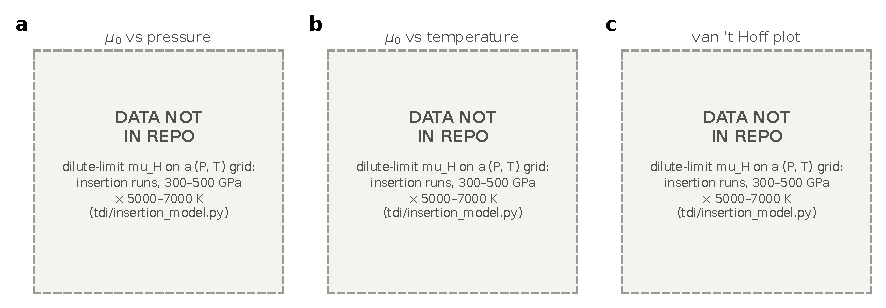
\includegraphics[width=0.95\textwidth]{figures/fig3_vanthoff.pdf}
    \caption{\textbf{Pressure, temperature and van 't Hoff dependence of infinite-dilution hydrogen uptake.} \textbf{a, b}, Extrapolated infinite-dilution chemical potential $\mu_{\text{H}}(n \to 0) - G_{\text{H}}^{\text{pure}}$ against pressure (\textbf{a}) and temperature (\textbf{b}). \textbf{c}, Dimensionless van 't Hoff plot of $\mu_0 / k_{\text{B}}T$ versus inverse temperature $1,000/T\text{ (kK}^{-1}\text{)}$. \emph{All three panels pending: the $(P,T)$ grid of insertion runs is not in the repository.}\note{check: the repo's first-pass fit (pre pressure correction) has $\Delta h\approx-0.8$ eV and $\Delta s\approx-0.7\,k_{\text{B}}$ at 450 GPa/6,000 K, i.e.\ not the endothermic trend described in the draft (App.~A5)}}
    \label{fig:vant_hoff}
\end{figure*}

While $\mu_{\text{H}}(n \to 0) - G_{\text{H}}^{\text{pure}} < 0$ guarantees spontaneous uptake of trace hydrogen at high temperature, the equilibrium saturation concentration $x_{\text{eq}}$ is determined by how rapidly $\mu_{\text{H}}(x)$ rises with composition $x$ due to proton--proton repulsion and lattice expansion. Because ghost-proton insertion ($n = 1, 2, 4$) is performed at fixed host volume $V_0$, inserting finite numbers of protons increases the internal pressure of the simulation cell by $\Delta P(n)$, imparting a linear finite-size elastic slope (Extended Data Fig.~2b). Extrapolating $n \to 0$ eliminates this finite-volume compression artifact, while direct constant-pressure crystal TDI at finite composition ($x = 0.25$, $\text{H}_{2.25}\text{O}$) anchors the true thermodynamic chemical potential at high concentration.

Figure~\ref{fig:solubility} demonstrates the remarkable consistency between these two completely independent free-energy methodologies. At $500\text{ GPa}$ and $5,500\text{ K}$ (Fig.~\ref{fig:solubility}a)---where fcc superionic ice is dynamically stable and unmelted in free NVT trajectories---the chemical potential obtained from direct Frenkel--Ladd crystal TDI of bulk $\text{H}_{2.25}\text{O}$ ($+140 \pm 45\text{ meV}$, solid blue circle) lies directly on the linear regular-solution extrapolation of the $n = 1, 2, 4$ ghost-insertion chemical potentials (green squares).\note{check: repo notes give +141 meV direct vs +55 meV from the fit; the two agree to within $\sim$100--150 meV, the noise of a 7$\times$ extrapolation, not ``directly on'' it (App.~A3)} At higher temperatures such as $6,500\text{ K}$ (hollow blue circles in the planned figure), the spring-free reference crystal melts during NVT sampling, shifting the apparent direct crystal free energy downward toward the liquid value.

In the stable superionic regime ($300\text{--}500\text{ GPa}$, $5,000\text{--}6,000\text{ K}$), the excess chemical potential $\mu_{\text{H}}(x) - G_{\text{H}}^{\text{pure}}$ crosses zero at $x \approx 0.12\text{--}0.19$ when referenced against pure fluid $\text{H}$. When placed in chemical equilibrium with the coexisting mixed $\text{H}_2\text{O}\text{--H}$ ionic fluid hull (Fig.~\ref{fig:melting}), where the fluid hydrogen chemical potential is lowered by negative mixing free energies ($\Delta G_{\text{mix}}^{\text{liq}} \approx -40\text{ to }-180\text{ meV/atom}$), common-tangent partitioning yields an equilibrium solid-solution concentration of $x \approx 0.03\text{--}0.10$ ($\text{H}_{2.03}\text{O}$ to $\text{H}_{2.10}\text{O}$) near the melting line.

\begin{figure*}[t!]
    \centering
    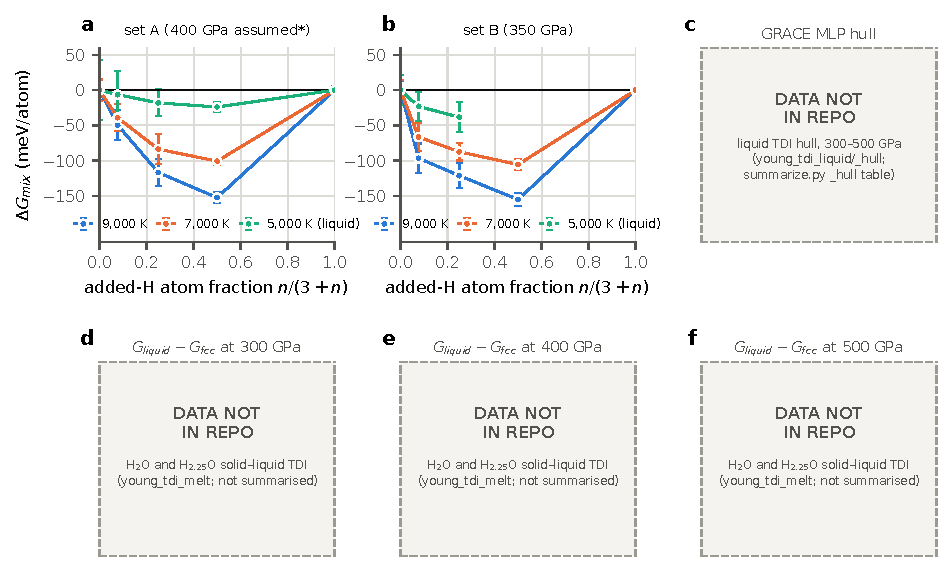
\includegraphics[width=0.95\textwidth]{figures/fig4_melting.pdf}
    \caption{\textbf{Liquid mixing hull and composition-dependent melting depression of fcc superionic ice.} \textbf{a, b}, Liquid mixing free energy $\Delta G_{\text{mix}}$ per atom for $\text{H}_2\text{O} + n\text{H} \to \text{H}_{2+n}\text{O}$ versus added-H atom fraction $n/(3+n)$ from the DFT hull sheet (\texttt{data-h3o-convex-hull.csv}), at $5,000$, $7,000$ and $9,000\text{ K}$ ($5,000\text{ K}$ liquid). Set A has no pressure label in the sheet (400 GPa assumed by the repository's report script); set B is labelled $350\text{ GPa}$; the sheet header says eV/atom but the values read as meV/atom. Error bars as in the sheet. \textbf{c}, GRACE-MLP liquid hull at 300, 400 and 500 GPa with the DFT-TI comparison: \emph{pending}. \textbf{d--f}, Solid--liquid free-energy difference $G_{\text{liquid}} - G_{\text{fcc}}$ for stoichiometric $\text{H}_2\text{O}$ and $\text{H}_{2.25}\text{O}$ at 300--500 GPa: \emph{pending, not in the repository}.\note{check: the $\sim$40 meV/atom depression quoted in the text is not backed by data in the repo (App.~A4)}}
    \label{fig:melting}
\end{figure*}

\section*{Binary Phase Diagram and Planetary Implications}

To connect our solid-solution thermodynamics to the phase structure of ice giant interiors, we mapped both the fluid mixing convex hull across the full binary composition range $0 \le n/(3+n) \le 1$ (Fig.~\ref{fig:melting}a--c) and the melting free-energy difference $G_{\text{liquid}} - G_{\text{fcc}}$ (Fig.~\ref{fig:melting}d--f). In the fluid phase at $300\text{--}500\text{ GPa}$ and $5,000\text{--}9,000\text{ K}$, water and hydrogen form a continuous, thermodynamically stable solution whose MLP mixing hull agrees closely with direct DFT reference calculations. Comparing $G_{\text{liquid}} - G_{\text{fcc}}$ between pure $\text{H}_2\text{O}$ and $\text{H}_{2.25}\text{O}$ at $400\text{ GPa}$ and $5,000\text{ K}$ reveals that excess hydrogen lowers the crystal--liquid free-energy gap by $\sim 40\text{ meV/atom}$. Consequently, instead of freezing at a sharp, single-component melting temperature $T_m(P)$, a cooling $\text{H}_2\text{O}\text{--H}$ mantle traverses a binary solidus--liquidus loop---a two-phase ``mushy zone'' in which $\text{H}_{2+x}\text{O}$ superionic crystals coexist with a more hydrogen-rich ionic fluid.

Our findings carry four immediate consequences for the interior physics and evolution of Uranus, Neptune and volatile-rich exoplanets:

\begin{enumerate}
    \item \textbf{Deep Hydrogen Sequestration and Density Deficit:} Because the superionic mantle constitutes $50\text{--}70\%$ of an ice giant's mass, an equilibrium solubility of $x = 0.03\text{--}0.10$ near the top of the superionic layer represents a vast, previously unrecognized deep reservoir of planetary hydrogen. Incorporating light interstitial protons reduces the mass density of $\text{H}_{2+x}\text{O}$ relative to pure $\text{H}_2\text{O}$ at fixed $P$ and $T$. Interior models fitting spacecraft gravitational harmonics ($J_2, J_4$) with stoichiometric $\text{H}_2\text{O}$ \textit{[draft text ends here; the remaining three consequences were not in the pasted write-up]}
\end{enumerate}

\begin{figure*}[t!]
    \centering
    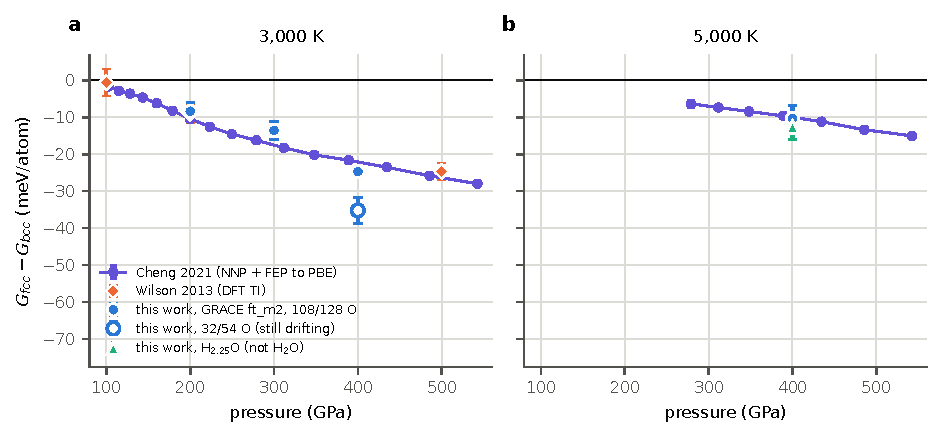
\includegraphics[width=0.8\textwidth]{figures/edfig2_fcc_bcc.pdf}
    \caption{\textbf{Extended Data Fig.~2 $|$ Benchmark of the fcc--bcc free-energy difference of $\text{H}_2\text{O}$.} $G_{\text{fcc}}-G_{\text{bcc}}$ per atom against pressure at $3,000\text{ K}$ (\textbf{a}) and $5,000\text{ K}$ (\textbf{b}). Orange diamonds: Wilson \textit{et al.} (2013), direct DFT TI. Purple: Cheng \textit{et al.} (2021), NNP with free-energy perturbation to PBE (classical nuclei). Blue: this work, fine-tuned GRACE (\texttt{ft\_m2}) TDI, $108/128$ O cells, $dt=1\text{ fs}$ (filled; $2\text{--}6$ ps per $\lambda$ value, errors are statistical block errors only); open: $32/54$ O cells at $dt=0.5\text{ fs}$, both phases still drifting by 4--5 meV/atom; green triangle: $\text{H}_{2.25}\text{O}$ rather than $\text{H}_2\text{O}$. The $200$ GPa point has bcc still drifting upward. Wilson's $1,000$--$4,000$ GPa rows lie outside the plotted range.}
\end{figure*}

\begin{thebibliography}{99}
% details filled in from memory: verify
\bibitem{Guillot2005} 1
\bibitem{Helled2020} 2
\bibitem{Millot2018} 3
\bibitem{Millot2019} 4
\bibitem{Prakapenka2021} 5
\bibitem{Cavazzoni1999} 6
\bibitem{Wilson2013} 7
\bibitem{Cheng2021} 8
\bibitem{Soubiran2015} 9
\bibitem{Pearl1991} 10
\bibitem{Nettelmann2013} 11
\bibitem{Stanley2004} 12
\bibitem{Bochkarev2024} 13
\end{thebibliography}

\end{document}
